% Drawing 79/14-1 -- folder 79, batch 14, archive page 275 (PDF page 276).
% Transcription: à gauche du NB, un double cône (bipyramide) sur un pentagone, arêtes cachées en pointillé.
% Kind: pentagonal bipyramid. Method 3 (encoded, rendered from the data). Status: ok.
% Notes: Double cone on a pentagon a b c d e, apexes N (top) and S (bottom); the hidden edges (to the back vertex e and the back side) dashed. Encoded as polyhedron/1: V 7, E 15, F 10, chi 2. Vertex names are ours (none on the page).
% Coordinates: 1 unit = 1 mm = 1/100 of the crop width (bbox in page fractions: [0.17, 0.38, 0.33, 0.53]).
% Redrawn by Claude (claude-opus-5-5), issue #73, 2026-11-07; not checked by a human; not compiled (no TeX in the session).
% Rights: reproduces part of the work -- behind RENDER_TRANSCRIPTS, never published by itself.
\documentclass[tikz,border=3pt]{standalone}
\usepackage{amsmath,amssymb}
\usetikzlibrary{patterns,arrows.meta}
\tikzset{pencil/.style={black!45}, struck/.style={black!35}, mark/.style={circle,draw,inner sep=1.3pt}, pt/.style={circle,fill,inner sep=0.9pt}, opt/.style={circle,draw,fill=white,inner sep=1.1pt}}
\begin{document}
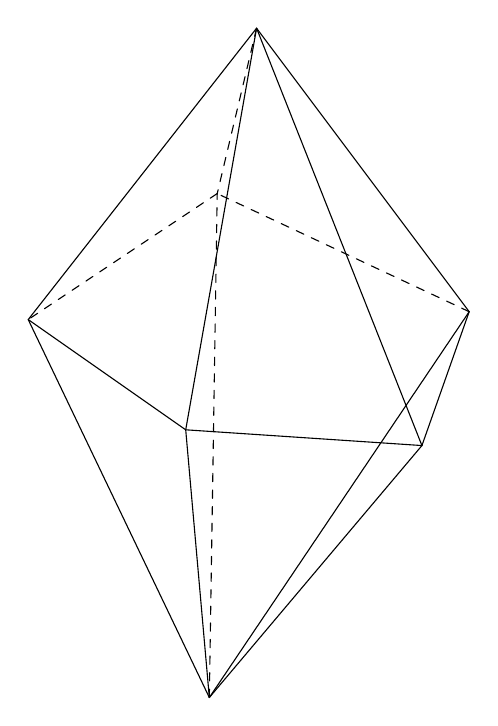
\begin{tikzpicture}[x=1mm,y=1mm,line cap=round,line join=round,font=\scriptsize]
\draw (10,-58) -- (30,-72);
\draw (30,-72) -- (60,-74);
\draw (60,-74) -- (66,-57);
\draw (39,-21) -- (10,-58);
\draw (39,-21) -- (30,-72);
\draw (39,-21) -- (60,-74);
\draw (39,-21) -- (66,-57);
\draw (33,-106) -- (10,-58);
\draw (33,-106) -- (30,-72);
\draw (33,-106) -- (60,-74);
\draw (33,-106) -- (66,-57);
\draw[dashed] (66,-57) -- (34,-42);
\draw[dashed] (34,-42) -- (10,-58);
\draw[dashed] (39,-21) -- (34,-42);
\draw[dashed] (33,-106) -- (34,-42);
\end{tikzpicture}
\end{document}
